\documentclass{beamer}
\mode<presentation>
{
  \usetheme{ldv}
  \setbeamercovered{transparent}
}

% Uncomment this if you're giving a presentation in german...
\usepackage[ngerman]{babel}

% ...and rename this to "Folie"
\newcommand{\slidenomenclature}{Folie}


\usepackage[utf8]{inputenc}
\usepackage{amsmath,amssymb,amsfonts}
\usepackage{times}
\usepackage{graphicx}
\usepackage{fancyvrb}
\usepackage{array}
\usepackage{colortbl}
\usepackage{tabularx}

% Uncomment me when you need to insert code
\usepackage{color}
\usepackage{listings}
\usepackage{minted}
\usepackage{algpseudocode}
% End Code

\usepackage{datetime}
\usepackage{tikz}
\usepackage{xcolor}
\usepackage{enumitem}

\usetikzlibrary{calc}
\usetikzlibrary{shapes.geometric}
\usetikzlibrary{decorations.pathreplacing}

\lstset{basicstyle=\ttfamily}

% Uncomment me when you need video or sound
% \usepackage{multimedia}
% \usepackage{hyperref}
% End video

% Header
\newcommand{\zwischentitel}{Woche 12}
\newcommand{\leitthema}{Tobias Eppacher}
\newcommand{\presdatum}{\formatdate{14}{7}{2025}}
% End Header

% Titlepage
\title{Grundlagen: Algorithmen und Datenstrukturen}
\author{Tobias Eppacher}
\date{\presdatum}
\institute{School of Computation, Information and Technology}
\subtitle{Woche 12}
% End Titlepage


% Slides
\begin{document}


% 1. Slide: Titlepage
\begin{frame}
	\titlepage
\end{frame}

% 2. Slide: TOC
\begin{frame}
	\frametitle{Inhalt}
	\tableofcontents[subsectionstyle=hide]
\end{frame}

\section{Aufgaben}

\begin{frame}
	\frametitle{Aufgabe 12.1 - Dirty Double Hashing}
	\scriptsize
	Für diese Aufgabe verwenden wir ein modifiziertes Double Hashing, welches beim Löschen
	von Elementen die abhängigen Kollisionen nicht neu hasht, sondern einfach einen “gelöscht”-
	Platzhalter einfügt.
	Die Größe der Hashtabelle ist $m = 11$. Die Schlüssel der Elemente sind die Elemente selbst.
	\begin{align*}
		h(x, i) & = (h_1(x) + i \cdot h_2(x)) \mod m \\
		h_1(x)  & = 3x \mod m                        \\
		h_2(x)  & = 1 + (x \mod 10)
	\end{align*}

	\begin{enumerate}[label=\textcolor{black}{\alph*)},align=left,leftmargin=*]
		\item Unter welchen zwei Umständen kann \lstinline{find} ergebnislos abbrechen?
		\item Können bei dieser Vorgehensweise die Platzhalter beim Einfügen überschrieben werden?
		\item Wir fügen $n > 0$ Elemente in eine anfangs leere Hashtabelle ausreichender Größe
		      ein und löschen diese wieder. Was ist die Worst-Case Laufzeit einer folgenden \lstinline{find}-Operation? Begründen Sie Ihre Antwort kurz.
		\item Führen Sie die folgenden Operationen aus. Tragen Sie die überprüften Hashwerte ein.
	\end{enumerate}
	\begin{align*}
		\text{\lstinline{insert}: } & \quad 4, 15, 6, 10 \\
		\text{\lstinline{delete}: } & \quad 4, 10        \\
		\text{\lstinline{insert}: } & \quad 10, 1
	\end{align*}

\end{frame}

\begin{frame}[t]
	\frametitle{Aufgabe 12.1 - Dirty Double Hashing (a-c)}
	\small
	\begin{enumerate}[label=\textcolor{black}{\alph*)},align=left,leftmargin=*,itemsep=5em]
		\item \lstinline{find}-Abbruchgründe?
		\item \lstinline{insert}: Platzhalter überschreiben?
		\item Worst-Case \lstinline{find} nach \lstinline{insert} und \lstinline{delete} von $n > 0$ Elementen?
	\end{enumerate}
\end{frame}

\begin{frame}
	\frametitle{Aufgabe 12.1 - Dirty Double Hashing (d)}
	\begin{table}
		\centering
		\small
		\begin{tabular}{c|c|c|c|c|c|}
			      & $4$ & $15$ & $6$ & $10$ & $1$ \\
			\hline
			$i=0$ &     &      &     &      &     \\
			\hline
			$i=1$ &     &      &     &      &     \\
			\hline
			$i=2$ &     &      &     &      &
		\end{tabular}
	\end{table}

	\begin{table}
		\centering
		\small
		\begin{tabular}{l|c|c|c|c|c|c|c|c|c|c|c}
			          & $0$ & $1$ & $2$ & $3$ & $4$ & $5$ & $6$ & $7$ & $8$ & $9$ & $10$ \\
			\hline
			ins($4$)  &     &     &     &     &     &     &     &     &     &     &      \\
			\hline
			ins($15$) &     &     &     &     &     &     &     &     &     &     &      \\
			\hline
			ins($6$)  &     &     &     &     &     &     &     &     &     &     &      \\
			\hline
			ins($10$) &     &     &     &     &     &     &     &     &     &     &      \\
			\hline
			del($4$)  &     &     &     &     &     &     &     &     &     &     &      \\
			\hline
			del($10$) &     &     &     &     &     &     &     &     &     &     &      \\
			\hline
			ins($10$) &     &     &     &     &     &     &     &     &     &     &      \\
			\hline
			ins($1$)  &     &     &     &     &     &     &     &     &     &     &      \\
			\hline
		\end{tabular}
	\end{table}
\end{frame}

\begin{frame}[t]
	\frametitle{Aufgabe 12.2 - Multiple Choice (a)}
	\small
	Wir erweitern den Bubblesort-Algorithmus, indem vor \textbf{jeder} Vergleichsoperation eine
	Funktion \lstinline{isSorted} aufgerufen wird. Diese überprüft, ob das gesamte Feld bereits
	sortiert ist, indem jedes Paar von benachbarten Elementen uberprüft wird. Dazu wird
	das gesamte zu sortierende Feld einmal komplett durchlaufen. Ist das Feld sortiert,
	wird das modifizierte Sortierverfahren sofort beendet.

	Es bezeichne $f$ die \textbf{Worst-Case}-Laufzeit des Original-Bubblesort-Algorithmus und $g$
	die des modifizierten Bubblesort-Algorithmus. Was gilt?
	\begin{flalign*}
		 & \Box \quad f \in \Theta(g)                                                       &  & \\
		 & \Box \quad f \notin \Theta(g) \text{, aber } f \in \mathcal{O}(g)                &  & \\
		 & \Box \quad f \notin \Theta(g) \text{ und } g \in \mathcal{O}(f)                  &  & \\
		 & \Box \quad \text{weder } g \in \mathcal{O}(f) \text{ noch } f \in \mathcal{O}(g) &  &
	\end{flalign*}
\end{frame}

\begin{frame}[t]
	\frametitle{Aufgabe 12.2 - Multiple Choice (b)}
	\small
	Kreuzen Sie in den Zeilen (1) bis (3) jeweils das stärkste passende Symbol an. D. h.
	wenn z.B. $\Delta = o$ (bzw. $\Delta = \Theta$) möglich ist, wählen Sie $\Delta = o$ (bzw. $\Delta = \Theta$) und nicht
	$\Delta = O$. Falls die Funktionen unvergleichbar sind, kreuzen Sie u. (”unvergleichbar“) an.
	Setzen Sie also in jeder Zeile genau ein Kreuz
	\begin{flalign*}
		 & \text{Bsp: } & n           & \in \Delta(n^2)            &  & \Box \ o \quad \Box \ \mathcal{O} \quad \Box \ \Theta \quad \Box \ \omega \quad \Box \ \Omega \quad \Box \ u. \\
		 & \text{(1) }  & 7 \log_2(n) & \in \Delta(4 \log_2(n^2))  &  & \Box \ o \quad \Box \ \mathcal{O} \quad \Box \ \Theta \quad \Box \ \omega \quad \Box \ \Omega \quad \Box \ u. \\
		 & \text{(2) }  & n^3         & \in \Delta(n^8 (n \mod 2)) &  & \Box \ o \quad \Box \ \mathcal{O} \quad \Box \ \Theta \quad \Box \ \omega \quad \Box \ \Omega \quad \Box \ u. \\
		 & \text{(3) }  & 4^n         & \in \Delta(2^{4n})         &  & \Box \ o \quad \Box \ \mathcal{O} \quad \Box \ \Theta \quad \Box \ \omega \quad \Box \ \Omega \quad \Box \ u. \\
	\end{flalign*}
\end{frame}

\begin{frame}[t]
	\frametitle{Aufgabe 12.2 - Multiple Choice (c \& d)}
	\small
	\begin{enumerate}[label=\textcolor{black}{\alph*)},align=left,leftmargin=*,itemsep=2em,start=3]
		\item Welche Aussagen sind wahr? \medskip \\
		      \begin{itemize}[label={}]
			      \item $\Box$ \, Jeder AVL-Baum ist zugleich ein binärer Suchbaum.
			      \item $\Box$ \, Jeder binäre Suchbaum ist zugleich ein Binärer Heap.
			      \item $\Box$ \, Jeder Binäre Heap ist zugleich ein AVL-Baum.
			      \item $\Box$ \, Jeder Binäre Heap ist zugleich ein binärer Suchbaum.
		      \end{itemize}
		\item Welche Operation muss in einem Binären Min-Heap beim Ausführen von \lstinline{decreaseKey}
		      (Verringern eines Schlüssel-Wertes) u.U. aufgerufen werden, um die Heap-Invariante wiederherzustellen? \medskip \\
		      \begin{tabular}{llll}
			      $\Box$ \lstinline{siftUp}   &
			      $\Box$ \lstinline{siftDown} &
			      $\Box$ \lstinline{deleteMin}     &
			      $\Box$ \lstinline{rotateLeft}
		      \end{tabular}
	\end{enumerate}
\end{frame}

\begin{frame}[t]
	\frametitle{Aufgabe 12.2 - Multiple Choice (e \& f)}
	\small
	\begin{enumerate}[label=\textcolor{black}{\alph*)},align=left,leftmargin=*,itemsep=1.5em,start=5]
		\item Die durchschnittliche Laufzeit von Algorithmen (\textit{Average Case}) ist
		      \begin{itemize}[label={},itemsep=3pt,align=left,leftmargin=*]
			      \item $\Box$ \, uninteressant, da man ausschließlich am \textit{Worst-Case} interessiert ist.
			      \item $\Box$ \, oft nur mit großem Aufwand zu berechnen.
			      \item $\Box$ \, stets am besten geeignet, um den passenden Algorithmus zu wählen.
		      \end{itemize}
		\item Der MergeSort-Algorithmus
		      \begin{itemize}[label={},itemsep=3pt,align=left,leftmargin=*]
			      \item $\Box$ \, ist für alle Eingaben schneller als jede gute Implementierung von InsertionSort.
			      \item $\Box$ \, ist für bestimmte Eingabeklassen signifikant schneller als eine deterministische Implementierung von Quicksort.
			      \item $\Box$ \, ist im Schnitt um einen in der Eingabe linearen Faktor schneller als Quicksort.
			      \item $\Box$ \, sortiert eine Eingabe im Best Case in linearer Zeit.
		      \end{itemize}
	\end{enumerate}
\end{frame}

\begin{frame}[t]
	\frametitle{Aufgabe 12.2 - Multiple Choice (g)}
	\small
	\begin{enumerate}[label=\textcolor{black}{\alph*)},align=left,leftmargin=*,itemsep=1em,start=7]
		\item Beim Hashing mit \textit{linear probing}
		      \begin{itemize}[label={},itemsep=3pt,align=left,leftmargin=*]
			      \item $\Box$ \, werden Elemente, deren Schlüssel auf den gleichen Wert gehasht werden, in einer Liste abgelegt.
			      \item $\Box$ \, ist die Hashfunktion nicht besonders wichtig, da auf ineffiziente Listen verzichtet wird.
			      \item $\Box$ \, ist das Löschen von Elementen kompliziert, da Löcher in der Hashtabelle das Auffinden von anderen Elementen verhindern können.
		      \end{itemize}
	\end{enumerate}
\end{frame}

\begin{frame}[t]
	\frametitle{Aufgabe 12.2 - Multiple Choice (h)}
	\small
	\begin{enumerate}[label=\textcolor{black}{\alph*)},align=left,leftmargin=*,itemsep=1em,start=8]
		\item Der PermutationSort-Algorithmus sortiert ein Feld, indem er die Elemente wiederholt
		      umordnet und jede so entstandene Anordnung auf Sortiertheit prüft. \\
		      Es werden systematisch alle möglichen Anordnungen durchprobiert. Wir gehen im Folgenden davon
		      aus, dass PermutationSort ein Feld ohne Duplikate sortiert.
		      \begin{itemize}[label={},itemsep=3pt,align=left,leftmargin=*]
			      \item $\Box$ \, Für die \textit{Worst-Case}-Laufzeit $f$ von PermutationSort gilt $f \in \mathcal{O}(n^4)$.
			      \item $\Box$ \, Für die \textit{Average-Case}-Laufzeit $f$ von PermutationSort gilt $f \in \Theta(n \ast n!)$.
			      \item $\Box$ \, Fur die \textit{Worst-Case}-Laufzeit $f$ von PermutationSort gilt $f \in \mathcal{O}(n^n)$.
			      \item $\Box$ \, Mit einer sehr geringen, positiven Wahrscheinlichkeit terminiert PermutationSort
			            für bestimmte Eingaben niemals.
			      \item $\Box$ \, PermutationSort hat eine lineare \textit{Best-Case}-Laufzeit.
		      \end{itemize}
	\end{enumerate}
\end{frame}

\begin{frame}
	\frametitle{Aufgabe 12.3 - Graph Algorithmen}
	\small
	Gegeben sei der folgende Graph. Bearbeiten Sie mit diesem folgende Teilaufgaben:
	\begin{enumerate}[label=\textcolor{black}{\alph*)},align=left,leftmargin=*,itemsep=0.75em]
		\item Nennen Sie die Reihenfolge, in der eine Tiefensuche, die bei Knoten $0$ gestartet wird,
		      die Knoten des Graphen besucht, wenn die Nachbarn eines Knotens in aufsteigender
		      Reihenfolge entsprechend der natürlichen Zahlenordnung bearbeitet werden.
		\item Nennen Sie die Reihenfolge, in der eine Breitensuche, die bei Knoten $0$ gestartet wird,
		      die Knoten des Graphen besucht, wenn die Nachbarn eines Knotens in aufsteigender
		      Reihenfolge entsprechend der natürlichen Zahlenordnung bearbeitet werden.
		\item Kann der Graph topologisch sortiert werden? Begründen Sie Ihre Antwort und nennen
		      Sie, falls möglich, die topologische Sortierung der Knoten, die sich aus der Reihenfolge
		      ergibt, in der die von Ihnen in Aufgabe a) durchgeführte Tiefensuche die Knoten fertig
		      bearbeitet hat.
	\end{enumerate}
\end{frame}

\begin{frame}
	\frametitle{Aufgabe 12.3 - Graph Algorithmen}

	\begin{figure}
		\centering
		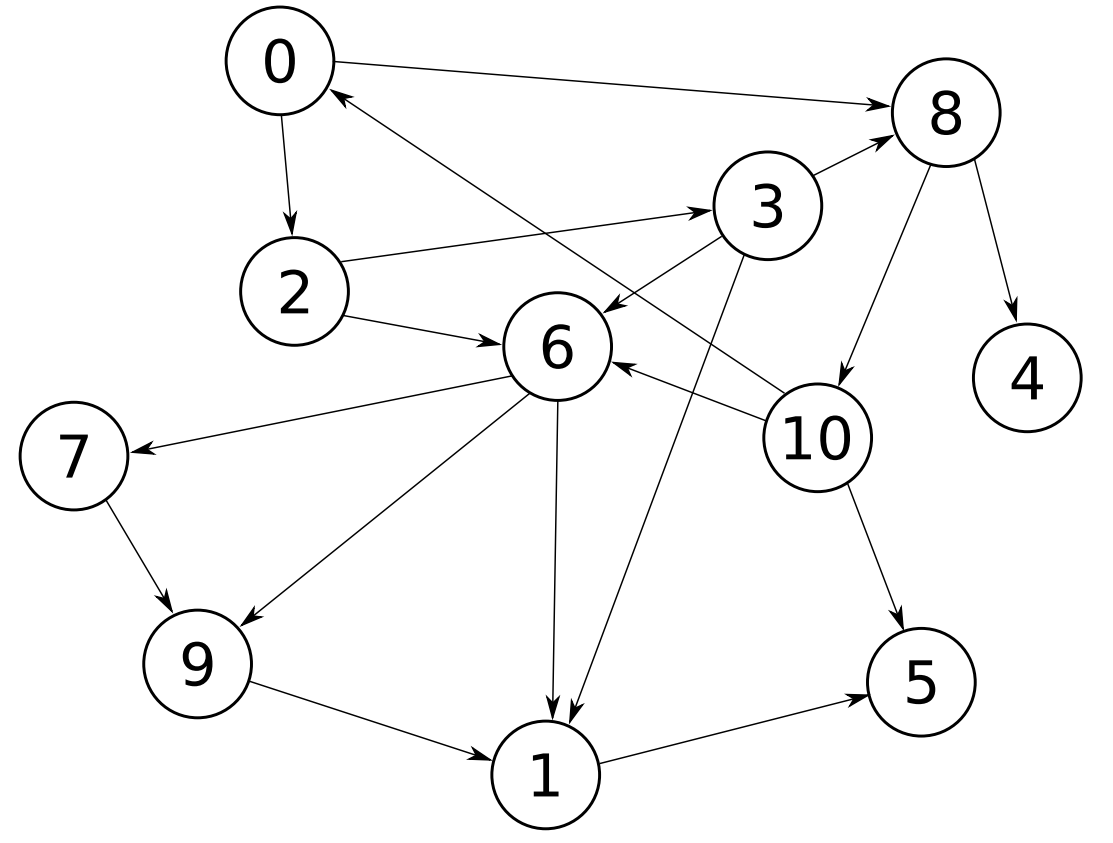
\includegraphics[width=0.7\textwidth]{images/graph12_3.png}
	\end{figure}
\end{frame}




\begin{frame}
	\frametitle{Aufgabe 12.4 - Netzwerk}
	\small
	Wir stellen uns ein soziales Netzwerk als Graph vor. In diesem Graph bilden die Personen des
	Netzwerks die Knoten. Sind zwei Personen befreundet, gibt es im Graphen eine ungerichtete
	Kante zwischen den entsprechenden Knoten.

	\begin{figure}
		\centering
		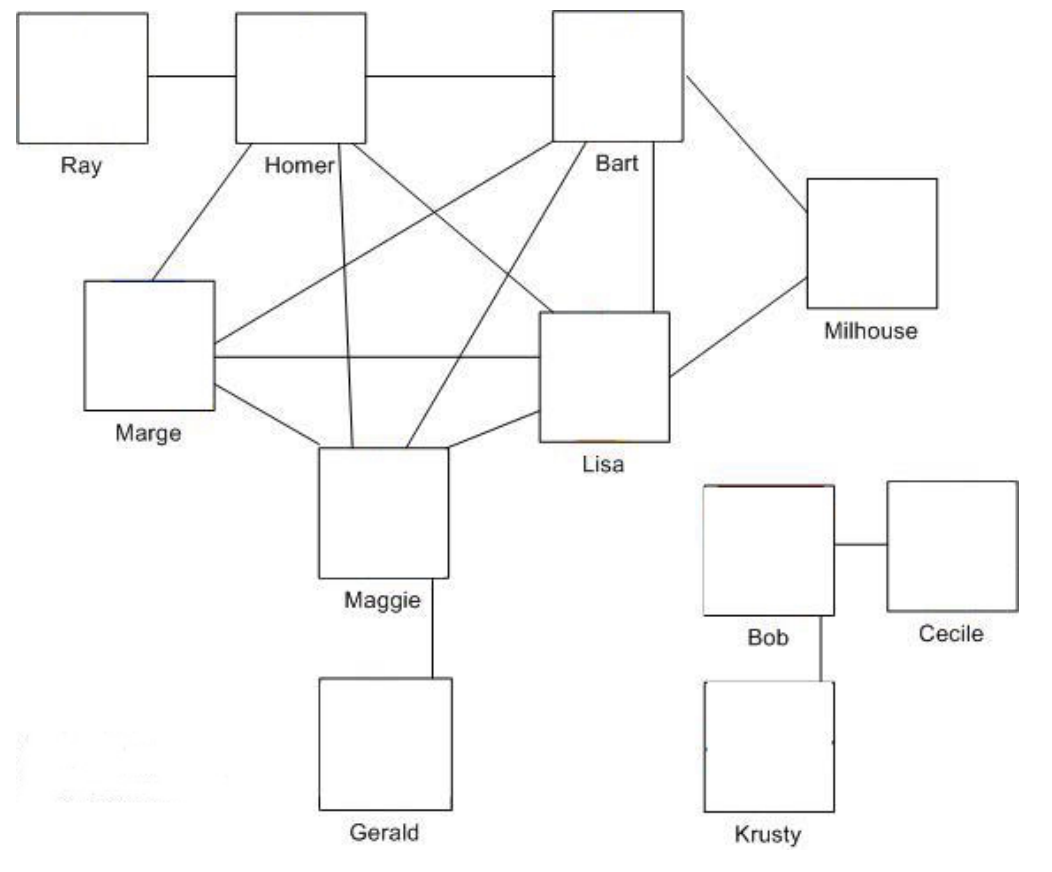
\includegraphics[width=0.6\textwidth]{images/graph12_4.png}
	\end{figure}
\end{frame}

\begin{frame}
	\frametitle{Aufgabe 12.4 - Netzwerk}
	\small
	\begin{enumerate}[label=\textcolor{black}{\alph*)},align=left,leftmargin=*,itemsep=0.75em]
		\item Wie kann man mit Hilfe der Tiefensuche feststellen, ob es einen Weg zwischen zwei
		      Personen in dem sozialen Netzwerk gibt? In diesem Fall sagen wir, dass sich diese
		      beiden Personen kennen.
		\item Überlegen Sie sich einen Algorithmus (basierend auf der Breitensuche), um festzustellen,
		      über wieviele Personen sich zwei Personen minimal kennen. Z.B. kennt Milhouse
		      Gerald minimal über zwei weitere Person (Lisa oder Bart und Maggie).
		\item Ergänzen Sie Ihren Algorithmus, so dass er eine kürzeste Verbindung ausgibt. Zum
		      Beispiel für die Verbindung Milhouse - Gerald wird ”Milhouse - Bart - Maggie - Gerald“
		      ausgegeben.
	\end{enumerate}
\end{frame}

\begin{frame}[t]
	\frametitle{Aufgabe 12.4 - Netzwerk}
	\small
	\begin{enumerate}[label=\textcolor{black}{\alph*)},align=left,leftmargin=*,itemsep=0.75em]
		\item Wie kann man mit Hilfe der Tiefensuche feststellen, ob es einen Weg zwischen zwei
		      Personen in dem sozialen Netzwerk gibt? In diesem Fall sagen wir, dass sich diese
		      beiden Personen kennen.
		      ausgegeben.
	\end{enumerate}
\end{frame}

\begin{frame}[t]
	\frametitle{Aufgabe 12.4 - Netzwerk}
	\small
	\begin{enumerate}[label=\textcolor{black}{\alph*)},align=left,leftmargin=*,itemsep=0.75em,start=2]
		\item Überlegen Sie sich einen Algorithmus (basierend auf der Breitensuche), um festzustellen,
		      über wieviele Personen sich zwei Personen minimal kennen. Z.B. kennt Milhouse
		      Gerald minimal über zwei weitere Person (Lisa oder Bart und Maggie).
	\end{enumerate}
\end{frame}

\begin{frame}[t]
	\frametitle{Aufgabe 12.4 - Netzwerk}
	\small
	\begin{enumerate}[label=\textcolor{black}{\alph*)},align=left,leftmargin=*,itemsep=0.75em,start=3]
		\item Ergänzen Sie Ihren Algorithmus, so dass er eine kürzeste Verbindung ausgibt. Zum
		      Beispiel für die Verbindung Milhouse - Gerald wird ”Milhouse - Bart - Maggie - Gerald“
		      ausgegeben.
	\end{enumerate}
\end{frame}

\begin{frame}[t]
	\frametitle{Aufgabe 12.4 - Netzwerk (Zusatz)}
	\small
	\begin{enumerate}[label=\textcolor{black}{\alph*)},align=left,leftmargin=*,itemsep=0.75em,start=4]
		\item Für Interessierte: Überlegen Sie sich, wie man diese Aufgabe in einem gerichteten
		      Graphen lösen könnte. \\
		      Übertragen auf das gegebene Beispiel könnte man eine gerichtete Kante (Marge, Krusty) einfügen, denn Marge kennt Krusty,
		      dieser kennt Marge aber nicht. Wie findet man nun heraus, dass es zwischen zwei Personen sowohl eine
		      Verbindung in die eine Richtung, als auch eine in die andere Richtung gibt?
	\end{enumerate}
\end{frame}

\begin{frame}
	\frametitle{Aufgabe 12.5 - Klausurvorbereitung}

	Nächste Woche: Letztes Tutorium, nur zwei Aufgaben!

	\bigskip
	Schickt mir gerne konkrete Fragen zu Themen, die ihr noch nicht verstanden habt oder
	wo ihr noch unsicher seid.
\end{frame}

\section{E-Aufgaben}
\begin{frame}
	\frametitle{E-Aufgaben}
	\begin{itemize}
		\item Aufgabe 12.6 - Multiple Choice 2
		\item Aufgabe 12.7 - Rückblick: Radixsort
		\item Aufgabe 12.8 - Klausurvorbereitung: Lückencode
	\end{itemize}
\end{frame}

\section{Hausaufgaben}
\begin{frame}
	\frametitle{Hausaufgaben}
	\begin{itemize}
		\item Hausaufgabe 10 - Simple Hashing with Chaining \\
		      (Deadline: 16.07.2025)
		\item Hausaufgabe 11 - Double Hashing \\
		      (Deadline: 23.07.2025)
		\item Hausaufgabe 12 - Graphen \\
		      (Deadline: 30.07.2025)
	\end{itemize}
\end{frame}

\begin{frame}
	\textbf{Fragen?}
	\begin{itemize}
		\item Nach Übung gerne bei mir melden
		\item Tutoriumschannel oder DM an mich auf Zulip
		\item Vorlesungschannels von GAD auf Zulip (insbesondere bei Hausaufgaben)
	\end{itemize}

	\medskip
	\textbf{Feedback oder Verbesserungsvorschläge?} \\
	Gerne nach dem Tutorium mit mir quatschen oder DM auf Zulip

	\medskip
	\textbf{Bis nächste Woche!}
\end{frame}

% End Slides

\end{document}
